\subsection{Validação e Análise do IRS}

A medida encontra problemas de escala e comparabilidade. A construção do Índice de Qualidade da Representação (IQR) agrega quatro dimensões padronizadas no intervalo \([0,1]\). No entanto, a dimensão Representação apresentou distribuição extremamente concentrada próxima de zero, com médias próximas a 0,1 (Figura \ref{fig:irs_mean_distribution}) e mediana \(\approx 0{,}01\) (Figura \ref{fig:irs_median_distribution}), enquanto as demais dimensões exibem medidas centrais mais elevadas (Profissionalização \(\approx 0{,}28\); Representação Descritiva \(\approx 0{,}48\)). Esse desalinhamento, sob agregação por média simples, a RS tenha peso efetivo muito reduzido no IQR, ainda que capture um atributo substantivo distinto. Do ponto de vista estatístico, o problema não é a validade do construto RS, mas a assimetria e compressão da sua distribuição em \([0,1]\).

\begin{figure}[h!]
    \centering
    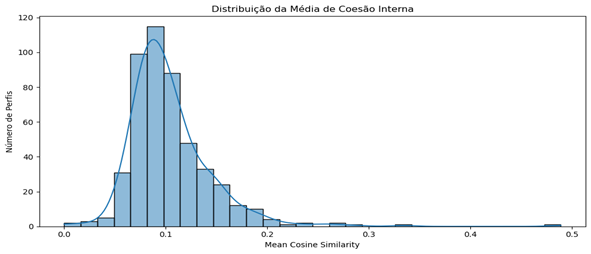
\includegraphics[width=0.8\textwidth]{figures/irs_Imagem1.png}
    \caption{Distribuição do IRS.}
    \label{fig:irs_mean_distribution}
\end{figure}

Os resultados se distribuíram em apenas metade do espaço total, com nenhum parlamentar tendo um escore superior a 0.5 no índice. Dentro desse espaço já reduzido, houve uma enorme concentração: 93,87\% dos deputados (n = 460) receberam escores entre 0.05 e 0.2. Encontra-se um cenário parecido, porém mais intenso quanto à concentração dos dados, quando analisamos os resultados da mediana: A mediana dos resultados de quase todo o universo se concentrou entre 0.0 e 0.02.

\begin{figure}[h!]
    \centering
    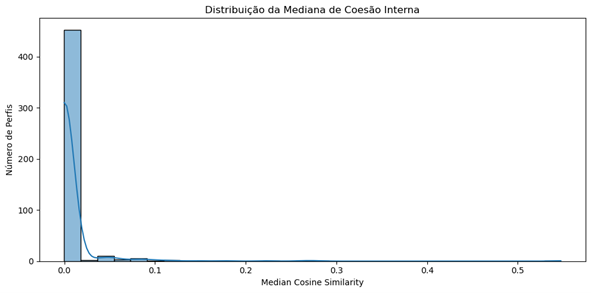
\includegraphics[width=0.8\textwidth]{figures/irs_Imagem2.png}
    \caption{Distribuição do IRS.}
    \label{fig:irs_median_distribution}
\end{figure}

Portanto, cremos que os resultados precisam ser normalizados de alguma forma. A ideia inicial é que o cálculo da LSA pode estar sendo influenciado pela variedade do volume de postagens dos parlamentares: 17,75\% (n = 87) dos deputados concentram 44,6\% das postagens (n = 136.759). Por mais que os escores médios não difiram muito entre os grupos, 0.096 e 0.098, apostamos que uma normalização anterior ao cálculo poderia tornar os resultados mais acurados.

Em resumo, o que preocupa é que, em meio a uma variedade grande de estratégias de comunicação e bases eleitorais dos deputados, os valores de coesão interna, além de estarem situados nas parcelas mais baixas do escore, se distribuem de maneira extremamente concentrada. 